\section{Auswertung}
\subsection{Messung des Erdmagnetfeldes und Isotopenzuordnung}
Zuerst wird die Stärke des gesamten Horizontal-Magnetfeldes aus der Abhängigkeit mit der Resonanzfrequenz für die beiden Rubidium-Isotope \ce{^{85}Rb} und \ce{^{87}Rb} bestimmt.
Das Magnetfeld besteht aus den Komponenten der Sweep-Spule und die der horizontalen Spule, die das Erdmagnetfeld in dieser Richtung kompensieren soll. Es besteht folgender Zusammenhang:
\begin{equation}
  B=B_\text{Sweep}+B_\text{Horizontal}
\end{equation}
Die Magnetfeldstärke $B$ ist aus der abgelesenen Stromstärke $I$ mithilfe des Zusammenhangs
\begin{equation}
B=\mu_0\frac{8IN}{\sqrt{125}R}
\end{equation}
berechnet worden. Hierbei ist $I$ der Strom, $N$ die Windungszahl der jeweiligen Helmholtzspule und $R$ der Radius der Spulen.
Abbildung \ref{fig:typSignalbild} zeigt einen typischen Signalverlauf. Zu sehen ist der tiefere Nullpunktspeak und die beiden Resonanzpeaks der Rubidium-Isotope.
\begin{figure}[H]
  \centering
  \includegraphics[width=0.45\textwidth]{Bilder/typSignalbild.jpg}
  \caption{Fotografie eines typischen Signalverlaufs bei \SI{100}{kHz}.}
  \label{fig:typSignalbild}
\end{figure}
In Tabelle \ref{tab:messwerte_resonanz} sind die gemessenen Positionen der Resonanzen in Abhängigkeit von der Frequenz $f_\text{RF}$ dargestellt. Eine lineare Ausgleichsrechnung der Form
\begin{equation}
  B=af_\text{RF}+b
\end{equation}
ist eingezeichnet.
Für die beiden Resonanzstellen ergeben sich die folgenden Regressionsparameter:
\begin{align*}
  a_1 = a_2 &= \SI{8,9 \pm 1,6 e-10}{\frac{MHz}{T}} \\
  b_1 = b_2 &= \SI{-1,6 \pm 0,9 e-4}{T}\\
\end{align*}
Die Messwerte für $f_\text{RF}=\SI{1}{MHz}$ erforderten eine so große horitontale B-Feldkomponente, das dieser Wert für den Graph und die anschließende Ausgleichsrechnung außer Acht gelassen wird.
\begin{table}[h]
  \centering
  \caption{Resonanzpositionen abhängig von der RF-Frequenz.}
  \label{tab:messwerte_resonanz}
  \begin{tabular}{S[table-format=1.1] S S S S}
    {$f_\text{RF}$ / MHz} & {$I_1$ / 0,1 A} & {$B_\text{horizontal}$ / 0,3 µT} & {$I_2$ / 0,1 A} & {$B_\text{horizontal}$ / 0,3 µT}\\
    \midrule
    0.1 &  0,35 &   0,0 & 0,44 & 0,0\\
    0.2 &  0,52 &   0,0 & 0,69 & 0,0\\
    0.3 &  0,69 &   0,0 & 0,95 & 0,0\\
    0.4 &  0,86 &  0,0 & 1,20 & 0,0\\
    0.5 &  0,68 &  1,5 & 1,10 & 1,5\\
    0.6 & 0,78 &  2,01 & 1,24 & 2,01\\
    0.7 & 0,91 &  2,01 & 1,49 & 2,01\\
    0.8 & 1,08 &  2,01 & 1,74 & 2,01\\
    0.9 & 1,24 &  2,01 & 2,00 & 2,01\\
    1.0 & 0,96 &  4,11 & 1,79 & 4,11\\
  \end{tabular}
\end{table}
\begin{figure}[H]
  \centering
  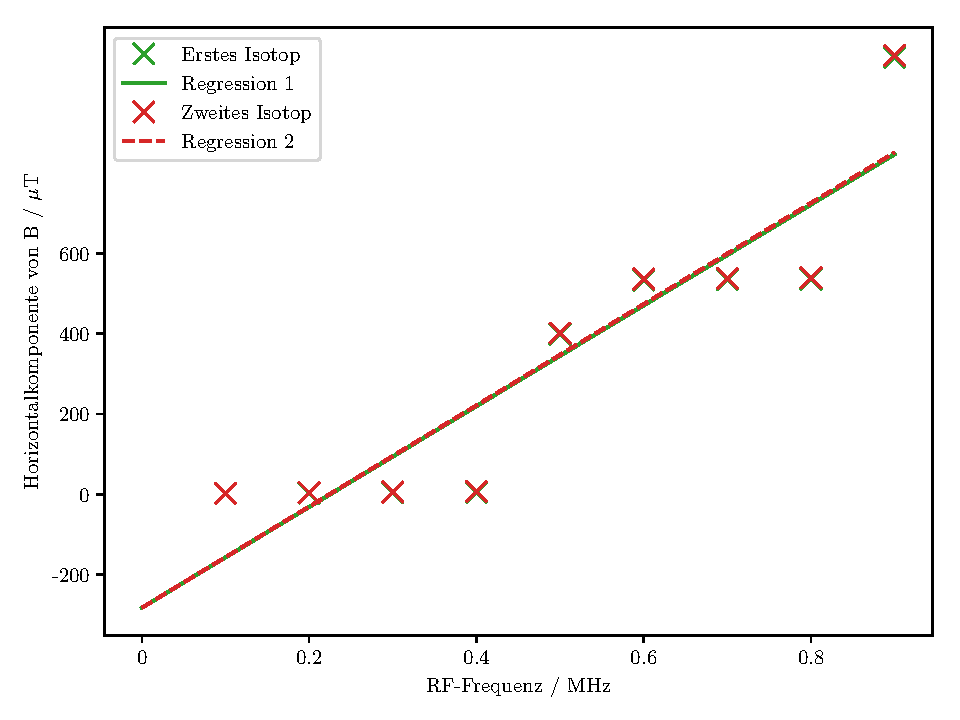
\includegraphics[width=0.8\textwidth]{Berechnung/resonanz.pdf}
  \caption{Magnetfeldstärke $B$ der Resonanzen in Abhängigkeit der Frequenz $f_\text{RF}$.}
  \label{fig:resonanz}
\end{figure}
\subsection{Bestimmung der Landé-Faktoren und des zugehörigen Kernspins}
Für die Berechnung der Landé-Faktoren wird die Formel
\begin{equation}
  \omega_0=g_F\frac{\mu_B}{h}B_0\quad \text{mit}\quad a=\frac{h}{\mu_B}{g_F}
\end{equation}
nach den Landé-Faktoren $g_F$ umgestellt. Mit dem Planckschen Wirkungsquantum $h$ und $a$ als die Steigung der Ausgleichsrechnung ergibt sich:
\begin{align*}
  g_F&=\frac{h}{\mu_Ba}\\
  \Rightarrow g_{F_1}&= 0,081 \pm 0,015\\
  \Rightarrow g_{F_2}&= 0,080 \pm 0,014.
\end{align*}
Für die Berechnung des Kernspins wird als erstes der Faktor $g_J$ aus ???? bestimmt. Mit ??? lässt sich dann der Kernspin $I$ bestimmen. Mit $J,S=0,5,L=0$ QUELLE und Formel ???? ergibt sich sodann:
\begin{align*}
  I_1&= 11,9\pm2,0\\
  I_2&=12,0\pm2,2.
\end{align*}
Im Vergleich zu den Literaturwerten QUELLE
\begin{align*}
  \ce{^{85}Rb}&:\; I=\frac{5}{2}\\
  \ce{^{87}Rb}&:\; I=\frac{3}{2}
\end{align*}
Eine Zuordnung der Messwerte zu den jeweiligen Isotopen ist aufgrund der unaussagekräftigen Abweichungen nicht möglich.
\subsection{Berechnung des Isotopenverhältnisses}
Um das Isotopenverhältnis zu bestimmen wird mir dem Cursor des Oszilloskops die Aplituden wie sie in Abbildung \ref{fig:typSignalbild} zu sehen sind, abgelesen.
Es ergeben sich die Aplituden in Einheiten der Oszilloskop-Koordinatensystemstriche:
\begin{align*}
A_1&= 5,5\\
A_2&= 11,5\\
\Rightarrow =\frac{A_1}{A_2}&=\frac{11}{23}\approx 0,48.
\end{align*}
Für das Isotopenverhältnis in der Natur gilt:
\begin{align*}
\Rightarrow =\frac{A_1}{A_2}=\frac{28\%}{72\%}\approx 0,38.
\end{align*}
Das Verhältnis des Isotopengeschmischs im Aufbau ist also um $26,3\%$ größer als in der Natur vorliegend.
\subsection{Quadratischer Zeemann-Effekt}
Für eine Abschätzung des quadratischen Zeemann-Effekts wird mit dem Zusammenhang \eqref{eq:quadratisch} die Energiedifferenz der Niveaus berechnet.
Mit den maximal gemessenen magnetischen Feldstärken für die erste Resonanzstelle von $B=\SI{1088,78}{µT}$ und $B=\SI{1096,37}{µT}$ für die zweite, ergibt sich mit $m_F=3$ für \ce{^{85}Rb} und $m_F=2$ für \ce{^{87}Rb} und der entsprechenden Hyperfeinstrukturaufspaltung aus Formel \eqref{eq:thermisch} ergeben sich:
\begin{align*}
  W_1&= \SI{3,6 \pm 0,6 e-9}{eV}\\
  W_2&= \SI{3,6 \pm 1,6 e-9}{eV}.
\end{align*}
\subsection{Transiente Effekte}
Die ansteigende Kurve ist in Abbildung \ref{fig:signal1} und ein typisches Signalbild einer abfallenden Kurve in Abbildung \ref{fig:signal2} gezeigt. Die Periodendauern der Oszillationen sind in Abbildung \ref{fig:periodendauern} grafisch dargestellt.
Eine hyperbolische Ausgleichsrechnung der Form
\begin{equation}
  y=a+\frac{b}{x-c}
\end{equation}
ist eingezeichnet.
Für die Regressionsparameter der ersten Resonanz ergeben sich
\begin{align*}
  a_1&= \SI{0,033 \pm 0,014}{ms}\\
  b_1&= \SI{4,47 \pm 0,14}{V ms}\\
  c_1&= \SI{0,45 \pm 0,06}{V};
\end{align*}
für die der zweiten Resonanz
\begin{align*}
  a_2&= \SI{0,14 \pm 0,07}{ms}\\
  b_2&= \SI{4,6 \pm 0,9}{V ms}\\
  c_2&= \SI{-1,9 \pm 0,5}{V}.
\end{align*}
Daraus errechnet sich das Verhältnis von
\begin{equation*}
\frac{b_2}{b_1}=\frac{\ce{^{85}Rb}}{\ce{^{87}Rb}}=1,04 \pm 0,20
\end{equation*}
zwischen den Landé-Faktoren.
Dies entspricht einer Abweichung von $69,33\%$ von dem theoretischen Wert von 1,5\cite{anleitung}.
\begin{figure}[H]
  \centering
  \includegraphics[width=0.8\textwidth]{Berechnung/perioden.pdf}
  \caption{Periodendauern der Oszillationen in ABhängigkeit der RF-Amplituden.}
  \label{fig:resonanz}
\end{figure}
\begin{figure}
  \centering
  \begin{subfigure}{0.46\textwidth}
    \centering
    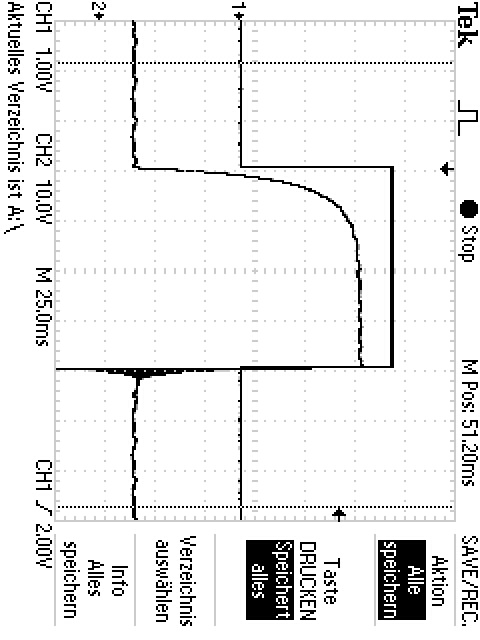
\includegraphics[angle=90, width=\textwidth]{bilder/flanke1.jpg}
    \caption{Ansteigende Flanke der Periodendauer für die erste Resonanzstelle.}
    \label{sub-abb:87}
  \end{subfigure}
  \qquad
  \begin{subfigure}{0.46\textwidth}
    \centering
    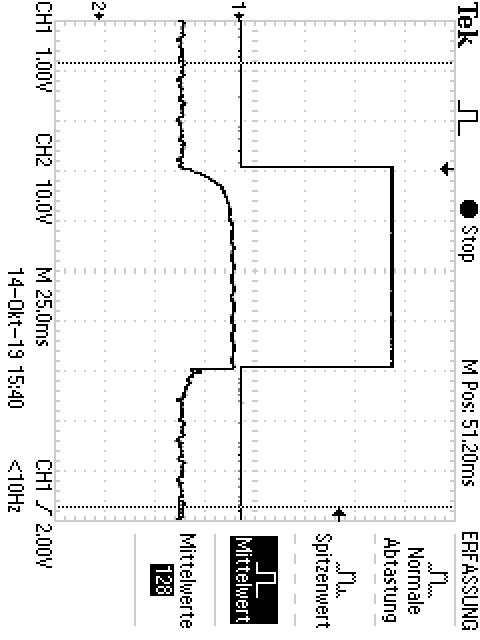
\includegraphics[angle=90, width=\textwidth]{bilder/flanke2.jpg}
    \caption{Ansteigende Flanke der Periodendauer für die zweite Resonanzstelle.}
    \label{sub-abb:85}
  \end{subfigure}
  \caption{Ansteigende Flanken der Periodendauern für beide Resonanzstellen entsprechend der Isotope.}
  \label{abb:ansteigende-flanken}
\end{figure}
